\section{Einf�hrung}
%
\subsection{Warum Versionierung?}
\begin{frame}
  \frametitle{Warum Versionierung?}
  \tableofcontents[currentsection,currentsubsection]
\end{frame}
%
\begin{frame}
  \begin{block}{Fragestellung}
    Welche gr��eren Probleme k�nnen bei der Programmierarbeit im Team mit mehreren Mitgliedern und Arbeitsger�ten auftreten?
  \end{block}
\end{frame}
%
\begin{frame}
  \frametitle{Sichere Indikatoren}
  \begin{itemize}
    \item "`Warum hast du gerade an der Datei rumgefummelt?? Da bin ich doch die ganze Zeit mit besch�ftigt"'
    \item<2->"`Gestern hat das Programm noch funktioniert, dann habe ich das neue Uber-Feature implementiert und nun ist es kaputt."'
    \item<3->"`Never touch a running system!"'
    \item<4->"`Als wir vor 3 Wochen mal probiert hatten, es ganz anders zu machen, hat zumindest das eine Feature funktioniert; aber keine Ahnung mehr wie das war"'
    \item<5->"`Wieso besteht diese Klasse zu 70\% aus auskommentiertem Code?"'
  \end{itemize}
\end{frame}
%
\begin{frame}
  \frametitle{Zusammenfassung}
  \begin{center}
    
\includegraphics[height=.75\textheight]{images/no_idea}
  \end{center}
\end{frame}
%
\begin{frame}
  \frametitle{Ziele der Versionierung}
  \begin{itemize}
    \item Protokollierung von Ver�nderungen
      \begin{itemize}
        \item Inklusive Metadaten wie Autor, Uhrzeit
        \item<2->\textbf{und Kommentar!}
      \end{itemize}
    \item<3->Wiederherstellung alter Zust�nde einzelner oder aller Dateien
    \item<4->Markierung von Zust�nden als Meilensteine oder Releases
    \item<5->Koordination gemeinsamer Arbeit
    \item<6->Parallele Entwicklungszweige f�r Features und verschiedene Releases
  \end{itemize}
\end{frame}
%
\begin{frame}
  \frametitle{L�sungen}
  \begin{itemize}
    \item Naive L�sungen
      \begin{itemize}
        \item Manuelles Speichern verschiedener Versionen von Dateien\\
          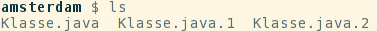
\includegraphics[width=.5\textwidth]{images/manuell}
        \item<2->Auskommentieren von altem Code\\
          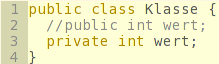
\includegraphics[width=.3\textwidth]{images/auskommentiert}
      \end{itemize}
    \item<3->Versionskontrolle
      \begin{itemize}
        \item CVS, SVN
        \item<4->F�r diese Veranstaltung: GIT
      \end{itemize}
  \end{itemize}
\end{frame}
%
%
\subsection{Schnappsch�sse \& Entwicklungszweige}
\begin{frame}
  \frametitle{Schnappsch�sse \& Entwicklungszweige}
  \tableofcontents[currentsection,currentsubsection]
\end{frame}
%
\begin{frame}
  \frametitle{Vokabular}
  \vspace{-7mm}
  \begin{description}
    \item[SCM] Source Control Management
    \item[Arbeitskopie]<2->Alle Dateien in einer bestimmten Version
    \item[Repository]<3->Enth�lt alle Versionen, Entwicklungszweige, etc.
    \item[Commit]<4->Version des Projekts oder einer Datei (auch Revision)
    \item[commit]<4->Erstellen eines neuen Commits im Repository
    \item[Branch]<5->Entwicklungszweig. Mindestens \texttt{master}-Branch
    \item[Tag]<6->Markierung eines Commits, z.B. als bestimmtes Release
    \item[Konflikt]<7->Kollidierende �nderungen
    \item[Merge]<8->Zusammenf�hrung der �nderungen mehrerer Commits
    \item[Graph]<9->Baum, der sich aus der Commit-Historie ergibt
    \item[Remote]<10->Server im Netz mit zentralem Repository
  \end{description}
\end{frame}
%
\begin{frame}
  \begin{center}
    
\includegraphics[height=\textheight]{images/problem}
  \end{center}
\end{frame}
%
%
\subsection{Arbeitsweise}
\begin{frame}
  \frametitle{Arbeitsweise}
  \tableofcontents[currentsection,currentsubsection]
\end{frame}
